%%%%%%%%%%%%%%%%%%%%%%%%%%%%%%%%%%%%%%%%%%%%%%%%%%%%%%%%%%%%%%%%%%%%%%%%%%%%%%%%%%%%%
%%%%%%%%%%%%%  Graph
%%%%%%%%%%%%%%%%%%%%%%%%%%%%%%%%%%%%%%%%%%%%%%%%%%%%%%%%%%%%%%%%%%%%%%%%%%%%%%%%%%%%%%%%%
\documentclass[../main.tex]{subfiles}
\begin{document}
\begin{figure}[!ht]
    \centering
    % 
\includegraphics[width=\columnwidth]{fig/graph_1.png}
    % \caption{An undirected graph}
    % \label{fig:graph_1}
    
        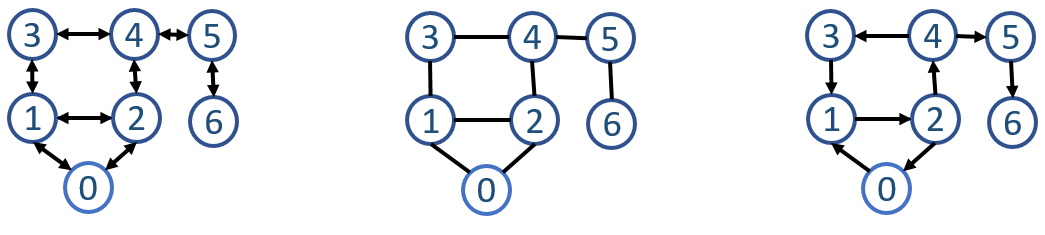
\includegraphics[width=\columnwidth]{fig/example_undirected_directed_graph.png}
    \caption{Example of undirected and directed graph: mark the vertices and edges}
    \label{fig:graph_2}
\end{figure}
Graph is a natural way to represent connections and reasoning between things or events. A graph is made up of \textit{vertices} (or nodes, points) are connected by \textit{edges} (arcs, or lines). A graph structure is shown in Fig.~\ref{fig:graph_2}.  There are many fields in that heavily rely on the graph, such as the probabilistic graphical models applied in computer vision, route problems, network flow in network science, link structures of a website in social media in computer science. 

In this chapter, we present graph as a data structure. However, graph is really a broad way to model problems; for example, we can model the possible solution space as a graph and apply graph search to find the possible solution to a problem.  So, do not let the physical graph data structures limit our imagination. 



As the first chapter related to graph, we mainly focus on explain related concepts, terminologies, graph representation, and the basic exhaustive search methods on real graph data structures:
\begin{itemize}
    \item Knowing the definition and the \textbf{terminologies} commonly used in Section~\ref{graph_terminology}. 
    \item \textbf{Representing the graph} data structures and implement these representation in Python in Section~\ref{graph_representation}.
    \item Learn the most basic graph search: Breath-first-search and Depth-first search in Section~\ref{sec_bfs}. 
\end{itemize}

\paragraph{Arrangement of Graph in the Book} Searching in graph which lies at the heart of the field of graph algorithms, therefore, we put effort in this book to explain the behavior, properties of them compared with a lot other books.  More advanced searching techniques and applications will be detailed in Chapter~\ref{chapter_non_linear_searching} in the part ~\ref{part_complete_searching}. And more advanced graph algorithms that build upon the basic searching techniques will be taught in Chapter ~\ref{chapter_advanced_non_linear_search} in part ~\ref{part_advanced_topics}.  And graph related questions instead will be categorized in Chapter ~\ref{chapter_graph_problem} in Part ~\ref{part_question}. 

%\section{Graph Traversal}
% \begin{figure}[h]
%     \centering
%     % 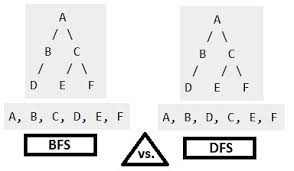
\includegraphics[width=0.6\columnwidth]{fig/dfs_bfs.png}
%     % \caption{BFS VS DFS}
%     % \label{fig:bfs_dfs}
%     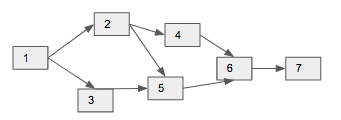
\includegraphics[width=0.6\columnwidth]{fig/example_graph.png}
%     \caption{Example Graph}
%     \label{example_graph}
% \end{figure}
% The breadth first search (BFS) and the depth first search (DFS) are the two algorithms used for traversing and searching a node in a graph. They can also be used to find out whether a node is reachable from a given node or not.   %In Fig.~\ref{fig:bfs_dfs} shows the BFS and DFS traverse ordering. Starting from a given vertex $u$, BFS will traverse all of its adjacency nodes $v_i$ and print out them, and then continue  to the adjacency nodes of $v_i$, while the DFS will traverse all of its adjacency nodes, but in a recursively way, which it recursively traverse the adjacency nodes of the current node untill reaching to a node that has no outgoing nodes.  

% Both BFS and DFS has a time complexity of $O(V+E)$ with adjacency list and $O(V^2)$ with adjacency matrix.



% A basic DFS and BFS implementation will only need state (1) and (3). While in some advanced extension of DFS and BFS, state (2) might be needed. Searching is an universal approach in problem solving. With searching, it literally search in the solution space and find the solutions. In this chapter, we focus on the basic Breadth-first and Depth-first Search algorithms executed on real graph data structure, and then exploring how to apply the DFS and BFS techniques on problem solution space, and introduce an optimized searching technique called \textit{Backtracking}.
% \begin{enumerate}
%     \item Breath-first Search in Section~\ref{sec_bfs}.
%     \item Depth-first Search in Section~\ref{searching_dfs}.
%     \item Graph Search for Problem Solving 
%     \item Backtracking
% \end{enumerate}

\paragraph{Graph in Interviews} Graph solution for some problems are most likely to be the naive solution, and it is a nice first step to give the naive algorithm design and analysis before moving on to more advanced solutions, such as divide and conquer, dynamic programming, or greedy algorithm. For some problems, graph search might be the only solution, so learning how to pruning the searching space with techniques like bidirectional search and backtracking would become handy. 

\section{Introduction and Terminologies}
\label{graph_terminology}
%%%%%%%%%%%%%%%%%%%%%%%%%%%%%%%%%%%%%%%%%%%%%%%%%%%%%%%%%%%%%%%%%%%%%%%%%%%%%%%%
% matrix and graph
%%%%%%%%%%%%%%%%%%%%%%%%%%%%%%%%%%%%%%%%%%%%%%%%%%%%%%%%%%%%%%%%%%%%%%%%%%%%%%%%%%%
% \section{Graphs}
% \label{chapter_graph_matrix}
Graph is a widely used data structure to model real-world problems. A graph  is a collection of \textit{vertices} and \textit{edges} (which connects two vertices). 



%%%%%%%%%%%%%graph representation%%%%%%%%%%%%%%%%%%%%%%%%%%


\end{document}